\documentclass[12pt,a4paper]{article}
\usepackage[utf8]{inputenc}
\usepackage[russian]{babel}
\usepackage[OT1]{fontenc}
\usepackage{amsmath}
\usepackage{amsfonts}
\usepackage{xcolor}
\usepackage{amsthm}
\usepackage{hyperref}
\usepackage{graphicx}
\usepackage{amssymb}
\usepackage{showkeys}
\usepackage{subcaption}
\author{Stepavly}
\newcommand{\bfline}[1]{\textbf{\underline{#1}}}
\newcommand{\Def}{\bfline{def} }
\newcommand{\R}{\mathbb{R}}
\newcommand{\n}{\bigbreak}
\newtheorem*{theorem*}{\bfline{Теорема}}

\begin{document}
\section{Линейные отображения.}
\subsection{Основные определения. Теорема о ранге и дефекте.}
\Def Линейное отображение $A$ --- функция $A$: $U \rightarrow V$, где $U, V$ - линейные пространства над $K$. Со свойствами:
\begin{enumerate}
	\item $\forall \lambda \in K$ $\forall v, u \in U$ \newline
		  $A(u+\lambda v)=A(u)+\lambda A(v)$
\end{enumerate}
Замечания:
\begin{enumerate}
	\item $A(u) = A u$ --- синтаксис.
	\item поточечно выполняются все свойства арифметических операций.
\end{enumerate}
Примеры:
\begin{enumerate}
	\item $\theta$ --- нулевое линейное отображение \newline
		  $\forall u \in V$ $\theta u = 0v$
		  
	\item $\varepsilon$ --- тождественное отображение

	\item $U = V = P_n$ --- многочлен степени $\leq n$. $A: U \rightarrow V$. \newline
		  $Ap = p'(t)$ --- дифференциальный оператор \newline
		  $A(p_1 + \lambda p_2) = (p_1 + \lambda p_2)' = p_1' + \lambda p_2'$

	\item $U = \mathbb{R}^n$, $V = \R^m$, $A=(a_{i j})$ $m \times n$. \newline
		  $A: x \in \R^n \rightarrow y = Ax \in \R^m$ \newline
		  $x_1 + \lambda x_m \in \R^n$, $A(x_1 + \lambda x_2) = A(x_1) + \lambda A(x_2)$

	\item Изоморфизм (взаимно однозначное соответствие)
\end{enumerate}
\Def Умножение линейного отображения на скаляр. \newline
$B = \lambda A$ \newline
$\forall u \in V$ $B(u) = \lambda A(u)$ \newline
\Def Сумма линейных отображений \newline
$C =A + B$ \newline
$\forall u \in V$ $C(u) = A(u) + B(u)$ \newline
$-A$ --- отображение противоположное $A$ \newline
\Def $A \in L(U, V)$
\begin{enumerate}
	\item $Ker\ A = \{v \in V\ |\  Au = \theta\}$ --- ядро линейного отображения
	\item $Im\ A = \{v = Au\ |\ \forall u \in U\}$ --- образ линейного отображения
\end{enumerate}
Замечание:
\begin{enumerate}
	\item $Ker\ A$ и $Im\ A$ - это линейные подпространства
\end{enumerate}
\Def Если:
\begin{enumerate}
	\item[$\bullet$] $Ker\ A$ конечномерное, то \newline
		$dim(Ker\ A) = def\ A$ --- дефект $A$
	\item[$\bullet$] $Im A$ конечномерное, то \newline
		$dim(Im\ A) = rg\ A$ --- ранг $A$
\end{enumerate}
\bfline{Утв}: $A$ изоморфизм  $U$, $V$ $\Leftrightarrow$
\begin{enumerate}
	\item $A \in L(U, V)$
	\item $Im\ A = V$
	\item $Ker\ A = \{0_v\}$ тривиально
\end{enumerate}
\bfline{Док-во}:
	$A$ изоморфизм $\Leftrightarrow$ взаимно однозначное и линейное \newline
	$\Rightarrow \left[
					\begin{array}{ll}
						\text{1) из определения} \\
						\text{2) взаимнооднозначно} \\
						\text{3) взаимнооднозначный ноль}
					\end{array}
				\right.$ \newline
	$\Leftarrow \left[
					\begin{array}{ll}
						\text{1) } Ker\ A = \{0\} \text{, значит инъективно, так как } v_1 = v_2 \Leftrightarrow u_1 = u_2 \\
						v_1 = A u_1, v_2 = A u_2 \\
						\underset{0}{\underbrace{v_2-v_2}} = \underset{\text{т.к. ядро тривиально}}{A u_1 - A u_2} = \underset{0}{\underbrace{A(u_1 - u_2)}} \\
						\text{2) } Im\ A = V \Leftrightarrow \forall v \in V:\ \exists u \in U\ Av = U \text{ --- сюръекция}
					\end{array}
				\right.$
\newline
\newline
\Def : $A \in L(U, V)$
\begin{enumerate}
	\item[$-$] инъективно, если $Ker\ A = 0$
	\item[$-$] сюръективно, если $Im\ A = U$
	\item[$-$] биективно, изоморфизм, если инъективно и сюръективно
	\item[$-$] эндоморфизм, линейный оператор, если $U = V$ \newline
		$End(V) = L(V, V)$
	\item[$-$] автоморфизм ($Aut(V)$), если эндоморфизм + изоморфизм
\end{enumerate}
\Def : Произведение линейных отоюражений
$$
U \underset{B}{\rightarrow} W \underset{A}{\rightarrow} V
$$
$
A \in L(W, V) \\
B \in L(U, W) \\
C = (A + B) \in L(V, U) \text{ --- композиция функций } A \text{ и } B. \\
A \cdot B = A \circ B \\
\forall u \in U\ (A \cdot B)(u) = A(B(u))
$
\newline
\bfline{Зам}: \begin{enumerate}
	\item $A$, $B$ изоморфизм, то $A \cdot B$ изоморфизм
	\item $(A_1 + A_2)B = B A_1 + B A_2$ \newline
		$B(A_1 + A_2) = B A_1 + B A_2$
	\item $A(BC) = (AB)C$
\end{enumerate}
Значит $End (U, V)$ --- алгебра с единицей и ассоциативностью. %TODO проверьте это, я не смог разобрать почерк
\newline
\Def : $A \in L(U, V)$ изоморфизм \newline
$
\forall u \in V\ \exists!\ u \in U: v = Au \\
A^{-1}: V \rightarrow U\ A^{-1}u = v
$ \newline
$A^{-1}$ линейное $A^{-1} A = \varepsilon u$, $A A^{-1} = \varepsilon v$. \newline
$A^{-1}$ изоморфизм. \newline
Если $A$ --- оператор, то $A^{-1}$ --- обратный оператор. \newline
\Def : $U_0 \in V$ $A \in L(U, V)$ \newline
Сужение $A$ на линейное подпространство $A|_{u_0}: U_0 \rightarrow V$ \newline
$\forall u \in U_0:\  A|_{u} v = A$ \newline
\bfline{Утв}: $A$ изоморфизм $\in L(U_1, V) \Rightarrow A|_{u_0}$ изоморфизм $\in L (U_0, Im\ A|_{u_0})$ \newline
Примеры:
\begin{enumerate}
	\item $0: V \rightarrow U$
		\begin{enumerate}
			\item[$-$] не сюръекция
			\item[$-$] не инъекция
			\item[$-$] эндоморфизм
			\item[$-$] не автоморфизм
		\end{enumerate}
	\item $\varepsilon: V \rightarrow V$ автоморфизм
	\item $A = \frac{d}{dt}$ $A: P_n \rightarrow P_n$
		\begin{enumerate}
			\item[$-$] не сюръекция
			\item[$-$] не инъекция
			\item[$-$] эндоморфизм
			\item[$-$] не автоморфизм
		\end{enumerate}
	\item $x \underset{\in \R^n}{\rightarrow} y = Ax \in \R^n$
		\begin{enumerate}
			\item[$-$] Если $rg A = n \Leftrightarrow$ инъекция и сюръекция
			\item[$-$] автоморфизм $\Leftrightarrow$ $rg A = n$
		\end{enumerate}
\end{enumerate}
\begin{theorem*}{(о ранге и дефекте отображений) \newline}
	$$A \in L(U, U)$$
	$$rg A + def A = dim U$$
\end{theorem*}
\bfline{Док-во}
\begin{figure}[h]
	\centering
	\begin{subfigure}[b]{0.25\linewidth}
		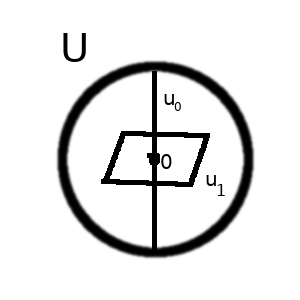
\includegraphics[width=\linewidth]{1.png}
		\caption{$U_0 = k + vA$}
	\end{subfigure}
	\begin{subfigure}[b]{0.25\linewidth}
		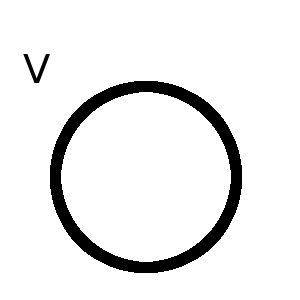
\includegraphics[width=\linewidth]{2.png}
		\caption{$U = U_0 \oplus U_1$}
	\end{subfigure}
	\begin{subfigure}[b]{0.25\linewidth}
		\caption{$U_1 \cap U_1 = \{0\}$}
	\end{subfigure}
\end{figure}
$\forall v \in U\ u = u_0 + v_1$ единственным образом \newline
$A u = A \underset{Ker A}{\underbrace{u_0}} + A u_1 = A u_1$. Значит $Im a = A V_1$ \newline
$A_1 = A|_{u_1}: u_1 \rightarrow Im A$, $A_1$ - изоморфизм. \newline
$U_1 \cong Im A \Leftrightarrow dim(U_1) = dim(Im\ a) \Leftrightarrow dim(Ker A) \neq dim(Im\ a) = dim(U)$ \newline
\bfline{Следствия}:
\begin{enumerate}
	\item $A \in L(U, V)$ эквивалентно:
		\begin{enumerate}
			\item $A$ --- изоморфизм
			\item $dim V = dim U = rg A$
			\item $dim U = dim V$, $Ker A = \{0\}$
		\end{enumerate}
	\item $A \in End(V)$ эквивалентно
		\begin{enumerate}
			\item $A$ --- изоморфизм
			\item $dim V = rg A$
			\item $Ker A = \{0\}$
		\end{enumerate}
\end{enumerate}
\subsection{Матрица линейного отображения. Изоморфизм алгебр. Преобразование матрицы линейного отображения при замене базиса.}
$A \in L(U, V)$ \newline
$\xi_1, \ldots, \xi_n$ --- базис $U$ \newline
$\eta_1, \ldots, \eta_m$ --- базис $V$ \newline
$\forall u \in U$ $u = \sum\limits_{i=1}^{n} u_i \xi_i$ \newline
$v = Au = A(\sum\limits_{i=1}^{n} u_i \xi_i)=\sum\limits_{i=1}^{n} u_i \underset{\overbrace{\text{достаточно определить это}}}{A \xi_i}$ \newline
$Im A = span(A \xi_1, \ldots, A \xi_n)$ \newline
$A \xi_i \in V$, $A \xi_i = \sum\limits_{i=1}^{m} a_{ij} \eta_i$ \newline
$A_i = 
	\left( 
	\begin{matrix}
		a_{1i} \\
		a_{2i} \\
		\vdots \\
		a_{mi}
	\end{matrix} 
	\right)$, $A = (A_1, \ldots, A_n)$ --- матрица линейного отображения. \newline
$\bullet$ Частный случай: \newline
$$
	A \in End(V) : \underset{e_1, \ldots, e_n}{V} \rightarrow \underset{e_1, \ldots, e_n}{V}
$$
$$
	\text{матрица линейного оператора}
$$
Пример:
\begin{enumerate}
	\item $\varepsilon: \underset{e_1, \ldots, e_n}{V} \rightarrow \underset{e_1, \ldots, e_n}{V}$ \newline
		$\varepsilon e_i = e_i \Rightarrow 
			\left(
			\begin{matrix}
				0 \\
				\vdots \\
				1 \\
				\vdots \\
				0
			\end{matrix}
			\right)
			\begin{matrix}
				\\
				\\
				\leftarrow i\\
				\\
				\\
			\end{matrix} \Rightarrow
			\left(
			\begin{matrix}
				1 & \ldots & 0 \\
				\vdots & \ddots & \vdots \\
				0 & \ldots & 1
			\end{matrix}
			\right)$
	\item $e : \underset{e'_1, \ldots, e'_n}{V} \rightarrow \underset{e_1, \ldots, e_n}{V}$ \newline
		$\xi e'_1 = e'_i = \sum\limits_{j=1}^{n} t_{ji}e_j \Rightarrow T_i = 
		\left(
		\begin{matrix}
			t_{1i} \\
			\vdots \\
			t_{ni}
		\end{matrix}
		\right)$ \newline
		$T$ --- матрица перехода $= T_{e \rightarrow e'}$
	\item Матрица поворота :(
	\item $A: P_2 \rightarrow P_2$, базис - $1, t, t^2$ \newline
		$A = \frac{d^2}{dt}$, $End(V) \cong M_{n\times n}$
\end{enumerate}
Изоморфизм ассоциативных, унитарных алгебр \newline
$U$ $\xi_1, \ldots, \xi_n$ $\forall u \in U \leftrightarrow u = 
	\left(
	\begin{matrix}
	u_1 \\
	\vdots \\
	u_n
	\end{matrix}
	\right)$ \newline
$V$ $\eta_1, \ldots, \eta_n$ $\forall v \in V \leftrightarrow v =
	\left(
	\begin{matrix}
	v_1 \\
	\vdots \\
	v_n
	\end{matrix}
	\right)$ \newline
$A \in L(U, V) \underset{(z, \eta)}{\leftrightarrow} A$ \newline
$\underset{\underset{\sum\limits_{j=1}^{m} v_j \eta_j \text{, } v_j \text{ - координаты}}{||}}{v} = Au = \sum\limits_{i=1}^{n} u_i A \xi_i = \sum\limits_{i=1}^{n} u_i \sum\limits_{j=1}^{m} a_{ji} \eta_i = \sum\limits_{j=1}^{m} \underset{\text{координаты}}{\underbrace{(\sum\limits_{i=1}^{n} u_i a_{ji}})} \eta_i$ \newline
Значит $v_j = \sum\limits_{i=1}^{n} a_{ji} u_i \leftrightarrow V = Au, \mathcal{V} = \mathcal{A} \mathcal{U}$ \newline
Примеры:
\begin{enumerate}
	\item $A$ поворот на угол $\alpha$ \newline
		$(i, j) \leftrightarrow A = 
			\left(
			\begin{matrix}
			\cos \alpha & -\sin \alpha \\
			\sin \alpha & \cos \alpha
			\end{matrix}
			\right)$
\end{enumerate}
\begin{theorem*}{(о преобразовании матрицы линейного отображения при замене базиса) \\}
$A \in L(U, V)$ \newline
$U$ $\xi = (\xi_1, \ldots, \xi_n)$, $\xi' = (\xi'_1, \ldots, \xi'_n)$ $A \underset{(\xi, \eta)}{\leftrightarrow} A$ \newline
$V$ $\eta = (\eta_1, \ldots, \eta_n)$, $\eta' = (\eta'_1, \ldots, \eta'_n)$ $A \underset{(\xi', \eta')}{\leftrightarrow} A'$ \newline
$A' = T^{-1}_{\eta \rightarrow \eta'} A T_{\xi \rightarrow \xi'}$
\end{theorem*}
\bfline{Док-во}: \newline
$$\begin{matrix}
\underset{\xi_1, \ldots, \xi_n}{U} & \overset{\overset{\mathcal{A}}{\rightarrow}}{\underset{A}{\leadsto}} & \underset{\eta_1, \ldots, \eta_m}{V} \\
e_v \uparrow \uparrow_{T_{\xi \rightarrow \xi'}} & & _{T^{-1}_{\eta \rightarrow \eta'}} \downarrow \ \uparrow e_v \\
\underset{\xi'_1, \ldots, \xi'_n}{U} & \underset{\mathcal{A}}{\overset{A'}{\rightarrow}} & \underset{\eta'_n, \ldots, \eta'_m}{V}
\end{matrix}$$
$\mathcal{A}^1 = \varepsilon_{v}^{-1} \mathcal{A} \varepsilon_{v} \leftrightarrow A^{-1} = T_{\eta \rightarrow \eta'}^{-1} A T_{\xi \rightarrow \xi'}$ \newline
\bfline{Замечание}:
$V = Au \underset{(\xi, \eta)}{\leftrightarrow} v = Au$ \newline
$V = Au \underset{(\xi', \eta')}{\leftrightarrow} V' = A' u'$ \newline
$v = T_{\eta \rightarrow \eta'} v'$, $u = T_{\xi \rightarrow \xi'} u'$ \newline
$T_{\eta \rightarrow \eta'} V\ = A T_{\xi \rightarrow \xi'} u'$ \newline
$v' = \underset{A'}{\underbrace{T^{-1}_{\eta \rightarrow \eta'} A T_{\xi \rightarrow \xi'}}} u'$
\subsection{Инварианты линейного отображения}
\Def : Инвариант --- свойство, которое сохраняется при определённых преобразованиях. \newline
Форма записи $\mathcal{V} = \mathcal{A}u \leftrightarrow V = Au$ инвариант относительно замены базиса. \newline
\Def : $A_{m \times n}$ \newline
$Im A = span(A_1, \ldots, A_n) = \{ \sum\limits_{i=1}^{n} \alpha_i A_i | \alpha_i \in K\} =\{ \underset{\underset{Ax}{||}}{Y} \in \R^m | x \in \R^n\}$ 'newline
$rg A = dim(Im A)$ \newline
$Ker A = \{ x \in \R^n | Ax = 0\} = \{ \text{множество решений СЛОУ}\}$ \newline
$dim(Ker A) = n - rg A = def A$ \newline
$rg A + def A = n$ --- аналог теоремы о ранге и дефекте \newline
\begin{theorem*}
$\forall A \in L(U, V)$ \newline
$rg \mathcal{A} = rg A$ \newline
$def \mathcal{A} = def A$ \newline
$rg$, $deg$ инварианты относительно выбора базиса
\end{theorem*}
\bfline{Док-во}: $\mathcal{A} \underset{(\xi, \eta)}{\leftrightarrow} A$ \newline
$\xi = (\xi_1, \ldots, \xi_n)$ --- базис $U$ \newline
$\eta = (\eta_1, \ldots, \eta_n)$ --- базис $V$ \newline
$In \mathcal{A} = span(A_{\xi_1}, \ldots, A_{\xi_n})$ \newline
$\mathcal{A}_{\xi_i} \leftrightarrow A_i$ --- координатный изоморфизм \newline
$] rgA = k$, $k$ столбцов линейно независимы. По свойствам изоморфизма среди $\mathcal{A}_{\xi_i}$ тоже $k$ линейно независимых, а остальные --- линейные комбинации $\Leftrightarrow$ $dim(Im A) = k$ \newline
$\underset{\underset{n}{||}}{dim U} = \underset{\underset{k}{||}}{rg \mathcal{A}} + def \mathcal{A}$ \newline
$def \mathcal{A} = n - k = def A$ \newline
\bfline{Следствия}: $\mathcal{A}$ изоморфизм $\Leftrightarrow$  $A$ невырождена ($\exists A^{-1}$), где $A$ --- матрица в некотором базисе. \newline
\bfline{Док-во}: изоморфизм $\Leftrightarrow$ $def A = 0$ $\Leftrightarrow$ $rg A = n$ $\Leftrightarrow$ $A$ - невырожденная. \newline
Определитель $V$ $e_1, \ldots, e_n$ \newline
$D$ --- $n$-форма, $D(e_1, \ldots, e_n) = 1$ \newline
$\xi_1, \ldots, \xi_n \in V$ $D(\xi_1, \ldots, \xi_n) = det(\xi_1, \ldots, \xi_n)$ \newline
$A \in End(V)$ --- линейный оператор \newline
\Def : $det A = det(\mathcal{A} e'_1, \ldots, \mathcal{A} e'_n)$ 
\begin{theorem*}
$det \mathcal{A}$ не зависит от базиса $e$, $det \mathcal{A} = det \mathcal{A}'$.
\end{theorem*}
\bfline{Док-во}: $V$ $e_1, \ldots, e_n$ \newline
$det \mathcal{A} = det(\mathcal{A} e_1, \ldots, \mathcal{A} e_n)$ \newline
$\mathcal{A} e_k = \sum\limits_{i_k = 1}^{n} i_k k e_{i_k}$ \newline
$A_k = \left(\begin{matrix}
A_{1 k} \\
\vdots \\
A_{n k}
\end{matrix}\right)$ \newline
$det \mathcal{A} = \sum\limits_{i_1=1}^{n} \sum\limits_{i_2=1}^{n} \ldots \sum\limits_{i_n=1}^{n} a_{i_1 1} a_{i_2 2} \cdot \ldots \cdot a_{i_n n} \cdot \underset{n\text{-форма}}{\underbrace{det(e_{i_1}, \ldots, e_{i_n})}}=$ \newline
$= \sum\limits_{\sigma=(i_1, \ldots, i_n)} a_{i_1 1} \cdot \ldots \cdot a_{i_n n} \cdot det(e_{i_1}, \ldots, e_{i_n})=$ \newline
$=\sum\limits_{\sigma} a_{i_1 1} \cdot \ldots \cdot a_{i_n n} \cdot det(e_{i_1}, \ldots, e_{i_n}) \cdot {(-1)}^{\sigma} = $\newline
$=\sum\limits_{\sigma} {(-1)}^{\varepsilon(\sigma)} a_{i_1 1} \cdot \ldots \cdot a_{i_n n} = det A$ \newline
Сменим базис, $e'_1, \ldots, e'_n$ --- базис $V$ \newline
$det \mathcal{A} = det T^{-1} \mathcal{A} T = det \mathcal{A}'$ (т.к. $T^{-1} T = E$). \newline
\Def : Матрицы $A$, $B$ называются подобными, если существует невырожденная $C$: $B = C^{-1} A C$. \newline
\bfline{Следствия}: $\forall f$ --- $n$-формы на $V$ \newline
$\forall \xi_i, \ldots, \xi_n$ $\forall \mathcal{A} \in End(V)$ \newline
$f(\mathcal{A} \xi_1, \ldots, \mathcal{A} \xi_n) = det \mathcal{A} \cdot f(\xi_1, \ldots, \xi_n)$ \newline
\bfline{Док-во}: $f(\mathcal{A} \xi_1, \ldots, \mathcal{A} \xi_n) = a(\xi_1, \ldots, \xi_n) = det(\xi_1, \ldots, \xi_n) \cdot a(e_1, \ldots, e_n)=$ \newline %А точно $a$ ?TOFIX?
$=det(\xi_1, \ldots, \xi_n) f(\mathcal{A} e_1, \ldots, \mathcal{A} e_n)=\left[ \mathcal{A} e_k = \sum\limits_{i_k=1}^{n} a_{i_k k} e_{i_k}\right]=$ \newline
$=det(\xi_1, \ldots, \xi_n) \sum\limits_{\delta} {(-1)}^{\varepsilon(\delta)} a_{i_1 1} \cdot \ldots \cdot a_{i_n n} \cdot f(e_1, \ldots, e_n) =$ \newline
$=det(\xi_1, \ldots, \xi_n) f(e_1, \ldots, e_n) det \mathcal{A} = det \mathcal{A} \cdot f(\xi_1, \ldots, \xi_n)$ \newline
\bfline{Замечание}: \newline
$A B = (A B_1, \ldots, A B_n)$ \newline
$det(AB) = det(A B_1, \ldots, A B_n) = det(A) \cdot det(B_1, \ldots, B_n) = det A \cdot det B$. \newline
\bfline{Следствие 2}: $\mathcal{A}, \mathcal{B} \in End(V)$ \newline
$det (\mathcal{A} \cdot \mathcal{B}) = det \mathcal{A} \cdot det \mathcal{B}$ \newline
\bfline{Следствие 3}: $\mathcal{A} \in Ant(V) \Leftrightarrow det \mathcal{A} \neq 0$, $det \mathcal{A}^{-1} = \frac{1}{det \mathcal{A}}$ \newline
\bfline{Утверждение}: $A, B$ подобные $\Rightarrow tr A = tr B$. \newline
\bfline{Док-во}: $A, B$ подобные $\Rightarrow$ \newline
$\exists C$: $C^{-1} A C = B$ \newline
$tr B = \sum\limits_{i=1}^{n} b_{i i} = \sum\limits_{i=1}^{n} \sum\limits_{j=1}^{n} C^{-1}_{ij} {(AC)}_{ji}=$ \newline
$=\sum\limits_{i=1}^{n} \sum\limits_{j=1}^{n} \sum\limits_{k=1}^{n} C^{-1}_{ij} a_{jk} C_{ki} = \sum\limits_{j=1}^{n} \underset{\delta_{ki}}{\underbrace{\sum\limits_{k=1}^{n} a_{jk} \sum\limits_{i=1}^{n} C_{ki} C^{-1}_{ij}}}=$ \newline
$=\left[ \delta_{kj}=
	\left[
	\begin{matrix}
		1, k=j \\
		0, k \neq j
	\end{matrix}\right]\right]=
\sum\limits_{k=1}^{n} a_{kk} = trA$ \newline
\Def : $tr \mathcal{A} = tr A$ \newline
$tr A$ не зависит от выбора базиса \newline
\Def : $L \subset V$ $L$ инвариантно относительно $End(V)$, если $\forall u \in L$ $\mathcal{A} u \subset L$. \newline
\begin{theorem*}
$L \subset U$ $\mathcal{A} \subset End(U) \Rightarrow \exists$ базис $U$ такой, что матрица $A$ в этом базисе будет иметь вид \newline
$A=
	\left(
	\begin{matrix}
	A_1 & A_2 \\
	0 & A_3
	\end{matrix}
	\right)$ \newline
$A_{k\times k}$, где $k = dim L$
\end{theorem*}
\bfline{Док-во}: $L = span(e_1, \ldots, e_n)$ дополним до $V$ : $e_1, \ldots, e_k, e_{k+1}, \ldots, e_n$ \newline
$\mathcal{A} e_i \in L$, $\mathcal{A} e_i = \sum\limits_{m=1}^{k} a_{mi} e_m + \sum\limits_{m=k+1}^{n} 0 e_m$ \newline
$A_i = 
	\left(
	\begin{matrix}
	a_{1 i} \\
	\vdots \\
	a_{k i} \\
	0 \\
	\vdots\\
	0
	\end{matrix}
	\right)$ \newline
\bfline{Следствия}:
\begin{enumerate}
	\item $V = \bigoplus\limits_{i=1}^{m} L_i$, $L_i$ инвариантно по $\mathcal{A} \Rightarrow$ \newline
		$\exists$ базис пространства $V$, в котором матрица оператора имеет блочно-диагональный вид. \newline
		\bfline{Док-во}:  $L_i = span(e'_i, \ldots, e'^{i_k}_i$ \newline
		т.к. $\oplus$, то базис $V$ --- объединение базисов $L_i$
\end{enumerate}
\bfline{Следствие 2}: \newline
$
\begin{array}{r}
V = \bigoplus L_i, L_i\text{ --- инвариантно} \\
\mathcal{A} \in End(V)
\end{array} \Rightarrow Im a = \bigoplus\limits_{i=1}^{m} Im A|L_i
$ \newline
\bfline{Док-во}: \newline
$V = \bigoplus\limits_{i=1}^{m} L_i \Rightarrow \exists !$ представление $\forall \nu \subset U$ $\nu = \sum\limits_{i=1}^{m} \nu_i \in L_i$ \newline
$\underset{\subset Im \mathcal{A}}{\nu} = \mathcal{A}u = \sum\limits_{i=1}^{m} \underset{\in Im A|L_i}{\mathcal{A} u_i} \Rightarrow Im \mathcal{A} \subset \sum\limits_{i=1}^{m} Im A|L_i \Rightarrow Im \mathcal{A} \subset \sum\limits_{i=1}^{m} Im A|L_i$ \newline
$] \nu_i \in Im A|L_i$ $\nu_i = \mathcal{A} u_i$, $u_i \in L_i$ \newline
$\sum\limits_{i=1}^{m} v_i = \sum\limits_{i=1}^{m} \mathcal{A} u_i = \mathcal{A} \left( \sum\limits_{i=1}^{m} u_i \right) \in Im A$ \newline
$Im A = \sum\limits_{i=1}^{m} Im A|L_i$ \newline
$\nu_i \in Im A|L_i$ $\sum\limits_{i=1}^{m} \nu_i = 0$ \newline
$\nu_i = A u_i \Rightarrow A u_i \in L_i$ ($L_i$ инв.) $\Rightarrow \nu_i \in L_i$ и $\nu_i$ дизъюнктны, значит все $\nu_i=0$, значит $\mathcal{A}=\bigoplus\limits_{i=1}^{m} Im A|L_i$ 
\subsection{Собственные числа и вектора}
$\mathcal{A} \in End(V)$ \newline
\Def : $\lambda \in K$ собственное число линейного оператора $\mathcal{A}$, если $\exists v \in V \neq 0$, который называется собственным вектором, что $\mathcal{A} v = \lambda v$. \newline
$\exists v: \mathcal{A} v = \lambda v \Leftrightarrow (\mathcal{A} - \lambda \varepsilon) v = 0 \Leftrightarrow v \in Ker(\mathcal{A} - \lambda \varepsilon)$. \newline
\Def : $V_{\lambda} = Ker(A - \lambda \varepsilon) = \{\text{собственные вектора } V\}$ называется собственным подпространством. \newline
$\gamma(\lambda) = dim U_{\lambda}$ геометрической кратностью собственного числа \newline
$\gamma (\lambda)$ инвариантны относительно базиса ($Ker$ --- инвариант). \newline
$\lambda$ собственное число, $v$ собственный вектор $\Leftrightarrow Ker(\mathcal{A} - \lambda \varepsilon) \Leftrightarrow det(\mathcal{A} - \lambda \varepsilon)=0$ \newline
\Def : $\chi_A (t) = det(\mathcal{A} - t\varepsilon)$ --- характеристический многочлен \newline
$V$ $e_1, \ldots, e_n$ базис $\mathcal{A} \leftrightarrow A$ \newline
$\chi_{\mathcal{A}}(t) = det(\mathcal{A} - t\varepsilon) = det(A-t\varepsilon)$ \newline
$\chi_A(t) = det(A - t\varepsilon) = 
	\left(
	\begin{matrix}
	(a_{11}-t) & a_{12} & \ldots & a_{1n} \\
	a_{21} & (a_{22} - t) & \ldots & a_{2n} \\
	\ldots & \ldots & \ldots & \ldots \\
	a_{n1} & \ldots & \ldots & (a_{n n} - t)
	\end{matrix}
	\right)= $\newline
$={(-1)}^n t^n + {(-1)}^{n-1} \underset{tr A = tr \mathcal{A}}{\underbrace{(a_{11} + \ldots + a_{nn})}} t^{n-1} + \ldots + detA$ \newline
$det \mathcal{A} = \lambda_1 \ldots \lambda_n$, $\lambda_i$ --- корни $\chi_A(t)$ \newline
$\lambda \in K$ с.ч $\Leftrightarrow$ $\chi_A(\lambda) = 0)$ \newline
$K = \mathbb{C} \Rightarrow $ п.с.ч \newline
$K = \R \Rightarrow$ только вещественные корни будут собственными числами. \newline
\Def : множество всех чисел с учётом алгебраической кратности называется спектром линейного оператора. Спектр простой, если все собственные числа попарно различны. \newline
$det \mathcal{A} = \lambda_1 \ldots \lambda_n=0 \Leftrightarrow \exists \lambda = 0$ с.ч.
\begin{theorem*}
$\lambda$ с.ч. $\mathcal{A} \Rightarrow 1 \leq \gamma(\lambda) \leq \alpha(\lambda)$
\end{theorem*}
\bfline{Док-во}: $]  \gamma(\lambda) = k = dim V_{\lambda}$ \newline
$V_{\lambda}$ инвариантно относительно $\mathcal{A} \Rightarrow \exists$ базис: матрица будет иметь вид \newline
$A=
	\left(
	\begin{matrix}
		A_1 & | & A_2 \\
		- & + & - \\
		0 & | & A_3
	\end{matrix}
	\right)$ базис $= \underset{\text{собств. вектора}}{\underbrace{v_1, \ldots, v_k}}, v_{k+1}, \ldots, v_n$ \newline
$\mathcal{A}_{v_i}\subset V_{\lambda} = \lambda v_i \leftrightarrow
	A_i=
	\left(
	\begin{matrix}
		0 \\
		\vdots \\
		\lambda \\
		\vdots \\
		0
	\end{matrix}
	\right)$ \newline
	$\chi_{\mathcal{A}}(t) = det
	\left(
	\begin{matrix}
		\lambda-t & \ldots & 0 & | & & & \\
		\vdots & \ddots & \vdots & | & & & \\
		0 & \ldots & \lambda-t & | & A_2 & & \\
		- & - & - & + & - & - & - \\
		& & 0 & | & A_3 - t E & &
	\end{matrix}
	\right)=$ \newline
$=\left|
	\begin{matrix}
		\lambda - t & \ldots & 0 \\
		\vdots & \ddots & \vdots \\
		0 & \ldots & \lambda - t
	\end{matrix}
	\right| |A_3 - tE| = {(\lambda-t)}^k \chi_{A_3} (t)$ \newline
	$\lambda$ --- корень $\chi_A(\varepsilon)$ ратности не меняется $\Rightarrow \alpha(\lambda) \geq k \cdot \gamma(\lambda)$
\begin{theorem*}
$\lambda_1, \ldots, \lambda_m$ попарно различные с.ч. $\mathcal{A}$ \newline
$v_i, \ldots, v_m$ соответствующие им с.в. $\Rightarrow v_1, \ldots, v_m$ линейно независимы.
\end{theorem*}
\bfline{Док-во}: индукция \newline
\begin{enumerate}
	\item база $m=1$, ($\lambda_1, v_1$) лин. нез $V_1 \leq 0$
	\item ] верно для $m-1$
	\item ] $\lambda_1, \ldots, \lambda_m$ попарно различные.
\end{enumerate}
От противного, $\exists v_m = \sum\limits_{i=1}^{m-1} \alpha_i v_i$ \newline
$\sum\limits_{i=1}^{m-1} \alpha_i \lambda_m v_i = \lambda_m v_m = \overset{\leftarrow}{\mathcal{A}} \overset{\rightarrow}{v_m} = \sum\limits_{i=1}^{m-1} \alpha_i \mathcal{A} v_i = \sum\limits_{i=1}^{m-1} \alpha_i \lambda_i v_i$ \newline
$\sum\limits_{i=1}^{m-1} \alpha_i (\lambda_i - \lambda_m) v_i = 0$, значит $\alpha_i=0 \Rightarrow v_m=0$, противоречие \newline
\bfline{Следствие}: $\lambda_1, \ldots, \lambda_m$ попарно парличные с.ч. $\mathcal{A} \Rightarrow V_{\lambda_1}, \ldots, V_{\lambda_m}$ дизъюнктны \newline
\bfline{Док-во}: $v_1+\ldots+v_m=0$, $v_i \in V_{\lambda_i}$ \newline
Если бы хотя бы одно из слагаемых $\neq 0$, то это слагаемое с.в. $\Rightarrow$ противоречие с лин. незав. с.в. отвевечающих различным с.и. $\Rightarrow u_i : v_i = 0 \Rightarrow$ дизъюнктны.
\begin{theorem*}
$V = \bigoplus\limits_{i=1}^{m} L_i$, $L_i$ инвариантно относительно $\mathcal{A}$ \newline
$\mathcal{A}_i = \mathcal{A} |_{L_i} \cdot L_i \rightarrow \Rightarrow \chi_{A}(t) = \prod\limits_{i=1}^{m} \chi_{\mathcal{A}_i}(t)$
\end{theorem*}
\bfline{Док-во}: \newline
$A = 
	\left(
	\begin{matrix}
	\square & & \\
	& \square & \\
	& & \square
	\end{matrix}
	\right)$ --- очевидно.
\end{document}